\subsection{An exact negative-wSMI counterexample}
To show that negativity is a property of the population functional rather than only an estimation effect, modify the table in Eq.~\eqref{eq:zeroexample} to obtain $P=C/144$, where
\begin{equation}
C=\begin{pmatrix}
10&1&2&0&1&10\\
1&10&0&2&10&1\\
1&1&10&10&1&1\\
1&1&10&10&1&1\\
1&10&1&1&10&1\\
10&1&1&1&1&10
\end{pmatrix}.
\label{eq:counterexample}
\end{equation}
The four modified cells are all retained, and the modification preserves every row and column sum. Therefore $Q_{ij}=1/36$, $m=1/6$ and $z=2/3$ remain unchanged. Within $S$, two cells have count two, two have count zero and twenty have count one. Direct substitution gives
\begin{align}
W&=-\frac{11\log2}{36}\simeq-0.211795,\\
\operatorname{wSD}&=\frac{\log2}{36}\simeq0.019254.
\end{align}
The unweighted symbolic MI is approximately 0.551781 nats. All values are exact population quantities before decimal rounding. Dividing by $\log6$ gives the conventionally normalised measures and preserves the sign difference.

This distribution also has a finite time-series realisation. For each cell $(i,j)$, concatenate $C_{ij}$ paired blocks whose amplitudes equal the three ranks of symbols $i$ and $j$. With kernel three, delay one and stride three, the resulting 432-sample signals give exactly 144 paired symbols and reproduce $C$. Blocks are permuted together with a fixed random seed; no window crosses a block boundary. This construction establishes realisability for disjoint windows, and does not claim that an arbitrary ordinal table is attainable with overlapping windows in a stationary signal.

\subsection{Numerical checks and estimation bias}
We sampled 10,000 joint tables from a symmetric 36-cell Dirichlet distribution with concentration 0.4 per cell (seed 20261019). No table violated nonnegativity or the upper bound by unweighted symbolic MI, and 59 tables gave negative wSMI. The largest discrepancy in Eq.~\eqref{eq:correction} was $4.72\times10^{-16}$ nats. These checks test the implementation; the preceding proofs establish the distribution-wide results.

To examine the finite-sample null, we generated 200 independent pairs of independent standard Gaussian sequences at each of five lengths, with kernel three, delay one and overlapping windows. Population wSD is zero in this setting, but its mean plug-in estimate was 0.094992 nats for 100 samples and 0.000837 nats for 10,000 samples (Fig.~\ref{fig:synthetic}). Thus the proposed rescaling does not make the estimator unbiased. Overlapping windows are also not independent observations, so ordinary independent-cell uncertainty calculations should not be applied without justification.

\begin{figure*}[t]
\additioncolor
\centering
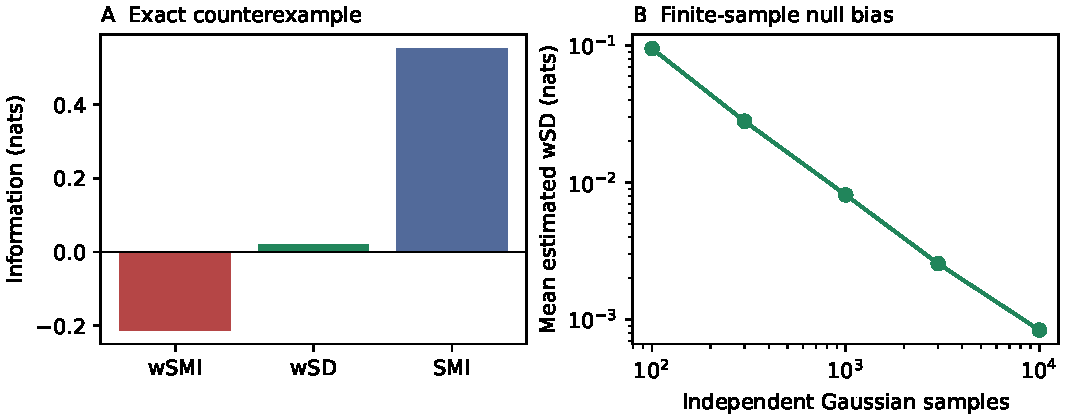
\includegraphics[width=.95\textwidth]{figures/synthetic_validation.pdf}
\caption{Exact and simulated validation. (A) The joint table in Eq.~\eqref{eq:counterexample} gives negative wSMI and positive wSD. (B) Mean estimated wSD for independent Gaussian sequences, using 200 replicates at each length. Its positive finite-sample bias decreases with sample length in this experiment.}
\label{fig:synthetic}
\end{figure*}

\subsection{Exploratory validation on public EEG}
We used the first five participants (S001--S005) and their two baseline recordings, eyes open (R01) and eyes closed (R02), from version 1.0.0 of the PhysioNet EEG Motor Movement/Imagery Dataset \cite{schalk2009dataset, schalk2004bci}. This fixed selection was made before inspecting the connectivity results. The recordings contain 64 EEG channels sampled at 160~Hz. Downloaded files were verified against the provider's SHA256 checksums; exact URLs and hashes are supplied with the analysis code.

Each recording was rereferenced to the common average and filtered continuously with a Butterworth bandpass designed using \texttt{scipy.signal.butter} with $N=4$ (an eighth-order bandpass), applied forward and backward using second-order sections. The lower cutoff was 0.5~Hz; the upper cutoff was $160/(3\tau)$~Hz. The primary delay was $\tau=4$ samples (25~ms; upper cutoff approximately 13.33~Hz); delays one and two were sensitivity analyses. The kernel was three throughout. The symbolic scale and lowpass convention follow the established wSMI methodology \cite{imperatori2019eeg}; this pilot does not reproduce a complete clinical wSMI preprocessing pipeline.

Five non-overlapping 10-second epochs began at 5, 15, 25, 35 and 45 seconds. Thus the first five seconds and all data from 55 seconds onward were excluded. Within each epoch, symbols were computed at every sample start, with no embedding across epoch boundaries. A pair was omitted if either ordinal window contained tied amplitudes; the joint table and both original marginals were computed from the same remaining pairs. There was no pseudocount or bias subtraction. All 2,016 distinct channel pairs were evaluated, giving 100,800 pair-epoch estimates for each delay. No channels or epochs were removed on the basis of connectivity values. There was no manual artifact rejection, ICA or source reconstruction, so artifacts and common-source effects remain possible explanations of individual estimates.

At the primary delay, wSMI was negative in 49,356 of 100,800 pair-epochs (48.96\%), whereas wSD ranged from 0.000813 to 0.621176 nats and never exceeded the corresponding unweighted symbolic MI. Each pair-epoch retained at least 1592 valid paired ordinal windows before the mask. Table~\ref{tab:negative} summarises the descriptive proportions by recording; Fig.~\ref{fig:eeg} shows all primary estimates. These pair-epochs share participants, electrodes and time, and must not be treated as 100,800 independent experimental units.

At delays one and two, respectively, 39.21\% and 49.23\% of pair-epochs gave negative wSMI; all wSD estimates again satisfied nonnegativity and the information bound. These proportions are descriptive and depend on the stated preprocessing and symbolic scale.

\begin{table}[t]
\additioncolor
\caption{Pair-epochs with negative wSMI at delay four. Each recording contributes 10,080 pair-epochs.}
\label{tab:negative}
\centering
\begin{tabular}{lrr}
\toprule
Participant & Eyes open (\%) & Eyes closed (\%)\\
\midrule
S001 & 57.3 & 53.5 \\
S002 & 57.1 & 42.1 \\
S003 & 65.5 & 57.2 \\
S004 & 53.7 & 26.3 \\
S005 & 40.0 & 37.0 \\
\bottomrule
\end{tabular}
\end{table}

For a reproducible illustration, the most negative primary wSMI occurred in S003R02, channels P5--PO7, in the epoch beginning at 15 seconds. Its wSMI was -0.154159 nats, while wSD was 0.063690 nats, with $m=0.166457$ and $z=0.616141$. The corresponding integer joint table is supplied as \texttt{eeg\_example\_counts.csv}. This example was selected after analysis to illustrate the sign contrast; it is not an independently selected hypothesis test.

As a descriptive null control, we circularly shifted one symbol sequence within each primary epoch for four prespecified homologous pairs (Fp1--Fp2, C3--C4, P3--P4 and O1--O2), using 99 shifts per pair-epoch, with seed 20261020. Shifts were sampled uniformly with replacement from integer offsets between 320 and $L-320$, where $L$ is the number of ordinal windows. This preserves each symbol sequence's cyclic structure while disrupting their original alignment. Across the 200 pair-epochs, the mean of the surrogate means was 0.018030 nats. The nonzero surrogate baseline reinforces the need for calibration; no significance or diagnostic claims are made. Circular shifts are an approximate control for dependent, potentially nonstationary data, not a guarantee of independence.

\begin{figure*}[t]
\additioncolor
\centering
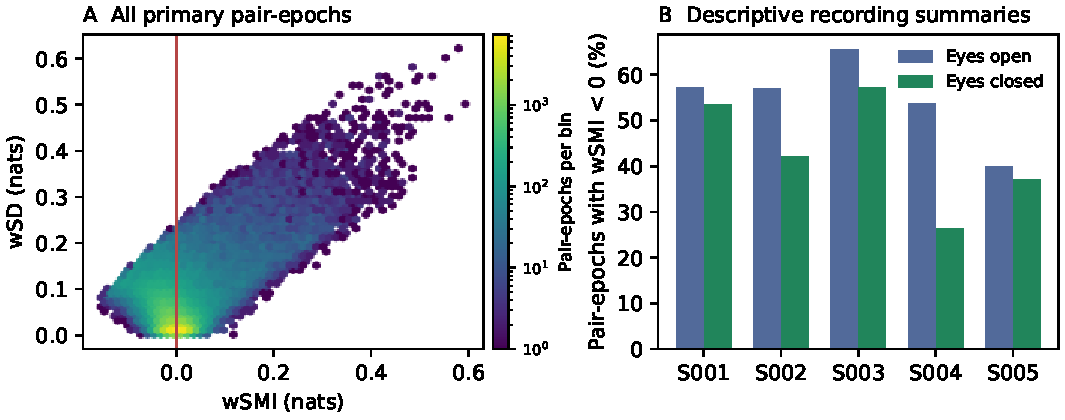
\includegraphics[width=.95\textwidth]{figures/eeg_validation.pdf}
\caption{Exploratory public-EEG results at kernel three and delay four. (A) All 100,800 pair-epoch estimates, with colour showing logarithmic bin counts and a vertical line at zero wSMI. (B) Descriptive percentages of negative wSMI within each recording. wSD remains nonnegative throughout; this numerical property is not evidence that all retained associations are physiological.}
\label{fig:eeg}
\end{figure*}
